\documentclass[11pt]{article}
\usepackage{titling}
% \usepackage[margin=1.5in]{geometry}
\usepackage{graphicx,caption,subcaption}
\usepackage{amsmath}
\usepackage{amssymb}
\usepackage{lipsum}
\usepackage{hyperref}
\usepackage[style=ieee, url=false]{biblatex}
\addbibresource{bibliography.bib}
\usepackage{array}
\newcolumntype{L}{>{\justarraybackslash}m{9cm}}

\begin{document}

\title{\bf Feature and Lazy Learning and the Jamming Transition in Artificial Neural Networks}
\author{
    % Hudson Cooper\\ % REDACT FOR SUBMISSION
    King's College London\\
    M.Sc.\ in Complex Systems Modelling
}
\date{\today}

\begin{titlingpage}
\maketitle
\begin{abstract}
Two distinct regimes of learning have been identified in modern, over-parameterized neural networks. In the ``lazy learning" regime, networks behave like linear models of features that are random but fixed at initialization, allowing precise asymptotic predictions of their generalization and convergence abilities. In the ``feature learning" regime, which has been implicated in the success of certain architectures such as the convolutional neural network (CNN), this simple description breaks down, making these networks much harder to analyze from a theoretical standpoint. To gain insight into this regime, we study linear models of varying degrees of random and trained features, in particular comparing their behavior near the so-called interpolation threshold, a critical point in the spectrum of model complexity that is associated with zero training loss and diverging test loss. While previous work has found that neural networks undergo a sharp ``jamming" phase transition at the threshold, we find this transition to be smooth for random features, with a sharp jamming transition only emerging with highly trained features.
\end{abstract}
\end{titlingpage}

\tableofcontents
\newpage

\section{Introduction}
Despite the remarkable success of neural networks in a variety of contexts such as vision, speech, natural language processing, drug discovery, and genomics \cite{lecunDeepLearning2015}, there is no cohesive theoretical explanation for this success; the understanding and design of these networks has been almost exclusively guided by empirical work. \\

Why are neural networks able to fit to and generalize from data so well? What criteria and design choices enable these abilities? These crucial questions remain open. Recent advances toward answering them have largely relied on the theoretical simplicity of an asymptotic regime known as ``lazy learning." This paper explores the limits of lazy learning's ability to adequately describe neural networks by comparing its behaviors to those of ``feature learning," a more complex and poorly understood regime that appears to be behind the successes of some of the most effective neural architectures, including convolutional neural networks. We in particular compare these two regimes in the vicinity of the interpolation threshold, a point which separates ``classical" statistical learning from ``modern" machine learning. This threshold is associated with diverging generalization error and critical behavior in the ability to fit to training data, baring many similarities to the ``jamming" phase transition in disordered solids. Our hope is that understanding the key differences between the two regimes around this critical point can lead to deeper understanding of neural networks in both regimes, allowing practitioners to design theoretically-motivated models with better convergence and generalization abilities.\\

The rest of the paper is organized as follows:
\begin{itemize}
    \item Section \ref{Background} provides an overview of the relevant background concepts and literature.
    \item Section \ref{Methods} describes the model that we use to investigate the behaviors of lazy and feature learning, additionally describing implementation details such as the data-set and optimization methods used throughout.
    \item Section \ref{Results} presents the main observations and findings.
    \item Section \ref{Discussion} contextualizes the findings and discusses their potential implications as well as the limitations and shortcomings of our approach.
\end{itemize}

\section{Background}
\label{Background}

\subsection{Double Descent: ``Classical" vs. ``Modern" Regimes}

The success of modern neural networks is in stark contrast with a main tenet of classical statistical learning: the so-called ``bias-variance trade-off." The bias-variance trade-off holds that more expressive models are more likely to find spurious patterns in data and generalize poorly to new samples, a behavior referred to as ``over-fitting." The trade-off implies that practitioners should seek to find the sweet-spot by building models that are ``as simple as possible, but no simpler." Neural networks, however, typically operate in a highly over-parameterized regime, containing many more parameters than there are data. Neural networks have been shown to be so highly expressive that they are able to interpolate and perfectly classify training data, even when labels have been replaced with pure noise \cite{zhangUnderstandingDeepLearning2017}. Classical statistical learning suggests that neural networks should therefore be extremely prone to over-fitting; however, despite their complexity and expressiveness, they are able to generalize extremely well in practice.\\

Recent work \cite{belkinReconcilingModernMachine2019} has characterised this phenomena in terms of the so-called ``double-descent" curve, visually represented in Figure \ref{doubledescent}. Two distinct regimes of model complexity are separated by the interpolation threshold, the point beyond which models are able to obtain perfect performance on training data. To the left of this threshold is the ``classical" or ``under-parameterized" regime, in which the bias-variance trade-off holds and generalization error follows a U-shaped curve, decreasing to a minimum before increasing to a peak at the interpolation threshold. Past this threshold, however, is the ``modern," ``interpolating," or ``over-parameterized" regime, in which the generalization error again decreases, with the global optimum being found deep in the over-parameterized regime, sometimes in the limit of infinite complexity. This double-descent phenomenology is far from unique to neural networks and has been observed in a variety of other model classes that are expressive enough to perfectly interpolate training data, including random forests, random feature models, and kernel machines \cite{ belkinReconcilingModernMachine2019, belkinUnderstandDeepLearning2018}. Several open questions remain about this modern regime: What are the sufficient conditions for training data to be well fitted and for interpolation to begin? What causes generalization to improve beyond this threshold?

\begin{figure}[ht]
\centering
\captionsetup{width=.8\linewidth}
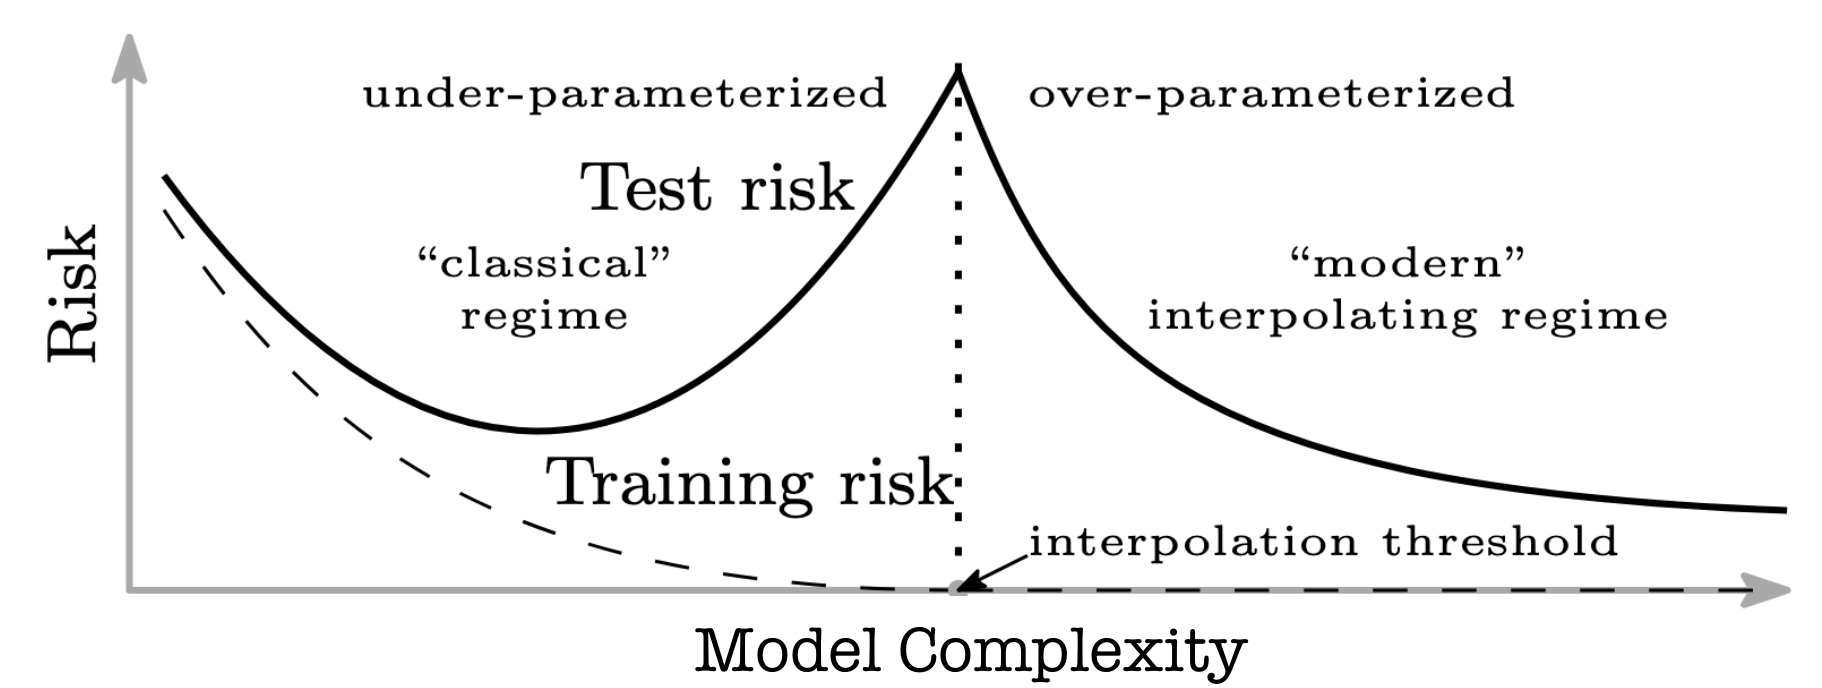
\includegraphics[width=0.8\textwidth]{docs/assets/double_descent_reconciling.png}
\caption{Visual depiction of the double descent curve, adapted from \cite{belkinReconcilingModernMachine2019}. The ``classical" U-shaped bias-variance trade-off is seen in the under-parameterized regime to the left of the interpolation threshold, and a second descent is seen in the over-parameterized regime to the right. Training error (``risk'') is represented with a dashed line, and test error is represented with a solid line.}
\label{doubledescent}
\end{figure}

\subsection{Lazy Learning in Over-Parameterized Networks}

By taking the limit as network width goes to infinity, a correspondence between wide, over-parameterized neural networks and the so-called ``lazy-learning" regime has been established, resulting in a recent flurry of theoretical progress. In particular, \cite{jacotNeuralTangentKernel2018} showed that gradient-descent on network parameters corresponds to gradient-descent on network outputs with respect to a kernel known as the ``Neural Tangent Kernel" (NTK). In the infinite width limit, the NTK converges to a deterministic limiting kernel that depends only on the network architecture, is independent of parameter initialization, and is constant throughout training. This limit is referred to as the ``lazy learning" limit because the constant NTK does not depend on the data-set. Although this correspondence is exact only in the infinite-width limit, experimental evidence across a variety of practical architectures shows good agreement between the limiting kernel machines and networks trained in the large but finite-width setting \cite{jacotNeuralTangentKernel2018}. Further work proved that the training dynamics of finite but over-parameterized networks rapidly converge to those of the corresponding limiting NTK \cite{allen-zhuConvergenceTheoryDeep2019}.\\

In the the lazy learning limit, network outputs can be expressed as a first-order Taylor expansion in the parameters about their randomly-initialized values at any time during training \cite{leeWideNeuralNetworks2019}. For a network $f_\theta$ with initial parameters $\theta_0$ and an initialization such that $f_{\theta_0} \approx 0$\footnote{Alternatively, one can define the network output to be $f_{\theta}(x) - f_{\theta_0}(x)$ done in \cite{chizatLazyTrainingDifferentiable2020}.}, we have that
\begin{equation}
    f_\theta(x) \approx \nabla_\theta \left.f_\theta(x)\right|_{\theta=\theta_0} \cdot (\theta - \theta_0)\,.
    \label{lazylinear}
\end{equation}
In other words, networks in the lazy-learning regime are linear models of random features given by the gradient of the network with respect to its parameters at initialization. The inner product in this random feature space converges to the limiting NTK as the number of parameters goes to infinity, suggesting that finite-width networks can be conceptualized as finite-rank approximations to the limiting kernel machine, connecting finite-width networks to the random features (RF) models proposed in \cite{rahimiRandomFeaturesLargeScale2008}.

\subsection{Theoretical Victories of Lazy Learning}

The lazy-learning regime offers a greatly simplified point of view from which to understand the training dynamics and convergence properties of overparameterized neural networks. Although training a neural network constitutes a large-scale non-convex optimization problem, the authors of \cite{allen-zhuConvergenceTheoryDeep2019} show that networks in the lazy regime are able to converge to global minima in polynomial time due to having ``nearly-convex" loss in a sufficiently large neighborhood around initialization, providing a reasonable explanation for the ability of over-parameterized networks to achieve near-zero loss.\\

In addition to explaining the convergence abilities of over-parameterized networks, lazy learning has also opened the generalization capabilities of networks near and above the interpolation threshold. As the interpolation threshold is approached from above, \cite{geigerScalingDescriptionGeneralization2019} argues that generalization error reaches a sharp peak due to random initialization in finite networks, causing the variance of the NTK to diverge. Above the interpolation threshold, lazy learning's connection to random-features (RF) models has allowed for rich asymptotic theory describing the generalization capabilities of these networks. RF models, as introduced in \cite{rahimiRandomFeaturesLargeScale2008}, are linear functions of pointwise nonlinearities applied to fixed random linear transformations of input data. They can be conceptualized as two-layer neural networks in which the first-layer weights (with width equal to the number of random features) are fixed at their randomly initialized values and the second layer weights are optimized freely. Note that for networks with a single hidden layer, the corresponding lazy linear model in Equation \eqref{lazylinear} can be exactly described as a RF model with independently distributed first-layer weights, but deeper networks require the introduction of potentially complex dependence structures \cite{chizatLazyTrainingDifferentiable2020}. For regression on random input data with linear or Gaussian-process target functions, the authors of \cite{meiGeneralizationErrorRandom2019} describe the generalization error of a RF model as the number of parameters $N$, the number of data $P$, and the input dimensionality $d$ are sent to infinity with their ratios fixed, and classification is similarly studied in \cite{dengModelDoubleDescent2020}. Remarkably, they are able to recover the full double-descent phenomenology in this simplified setting, including that the test error diverges at the interpolation threshold and that the global minimum of test error occurs in the infinitely over-parameterized regime, i.e. $N/P\rightarrow\infty$, as is predicted in \cite{belkinReconcilingModernMachine2019,belkinUnderstandDeepLearning2018} for kernel machines.\\

Building on the work of \cite{meiGeneralizationErrorRandom2019} and \cite{ geigerScalingDescriptionGeneralization2019}, which explores the role of initialization variance of the finite-rank NTK on generalization error, \cite{dascoliDoubleTroubleDouble2020} offers a ``modern" treatment of the bias-variance relationship beyond the interpolation threshold. This work disentangles the generalization error of an RF model into its constituent components of bias and multiple sources of variance, including the initialization variance of the random features, sampling variance of the data-set, and additive noise in the target variables. The theoretical predictions made in this simplified RF setting qualitatively match the empirical bias-variance decompositions made in \cite{nealModernTakeBiasVariance2019} for real neural networks, giving credibility to the RF model's ability to explain the behavior of neural networks in the overparameterized regime.

\subsection{Feature Learning}

Despite its success in explaining some of the crucial features of training and generalization in neural networks, the lazy learning perspective misses an important aspect of modern neural networks and deep learning: the role of ``feature learning."  The authors of \cite{chizatLazyTrainingDifferentiable2020} argue that the lazy-learning phenomenon occurs due to an implicitly chosen factor which controls how model parameters scale at initialization against network width. By making this scaling factor explicit, it is possible to force a network to train either in the lazy-learning regime or the so-called ``feature-learning" regime, in which the NTK is no longer constant and evolves throughout training in a manner dependent on the structure of the data. The feature-learning regime is also referred to as the ``mean-field" limit and is explored in some previous works, e.g. \cite{meiMeanFieldView2018}. While the dynamics of lazy learning can be described by a linear ordinary differential equation (ODE) of the network outputs and a constant NTK, the dynamics of feature-learning must be described by a more complex partial differential equation (PDE) which also depends on the empirical distribution of the activations of the hidden neurons. This increased complexity makes the convergence and generalization in the feature-learning regime much harder to study from a theoretical standpoint. And while networks in the lazy-learning regime are guaranteed to converge to a global minimum and have generalization error that is well-described by the asymptotics of RF models, it is not clear to what extent these properties and insights can be extended to networks in the feature-learning regime. \\

Lazy learning may be theoretically convenient, but it is not clear that it is a desirable regime in general. In particular, the role of feature learning in the ability of neural networks to generalize to unseen data is still poorly understood. Convolutional neural networks (CNNs) trained in the feature-learning regime have been found to outperform those trained in the lazy-learning regime, suggesting that lazy-learning does not account for the profound success of these networks \cite{chizatLazyTrainingDifferentiable2020}. On the other hand, \cite{geigerDisentanglingFeatureLazy2020} found lazy learning to out-perform feature learning (to a degree that depends on the data-set) in fully-connected networks (FCNs). This suggests that network architecture and the structure of data play important roles in determining which regime is better. It is still poorly understood how these architectural choices and their inductive biases with relation to data affect the quality of learned features. Understanding how these change the convergence conditions and generalization properties of neural networks remain important open questions in machine learning. 
 
\subsection{The Jamming Transition}

It is no surprise that highly expressive models, such as over-parameterized neural networks, have global optima associated with arbitrarily small training loss. Without appealing to lazy learning, however, it is highly non-trivial that direct optimization methods, such as stochastic gradient descent (SGD), are able to attain vanishing loss without getting stuck in local minima, due to generally non-convex and non-smooth loss landscapes. There are strong similarities between neural networks with their many parameters and models with many interacting components that are studied in the statistical-physics literature, in particular mean-field glassy systems. Glassy systems take an exponentially long time (in the degrees of freedom) to relax to global minima due to their extremely rough energy landscapes with many local minima. This suggests that neural networks should similarly converge to high and wide minima despite the existence of deeper local and global minima in their loss landscapes \cite{choromanskaLossSurfacesMultilayer}. In practice, however, SGD almost never encounters any such obstacles, and global minima are easily found \cite{goodfellowQualitativelyCharacterizingNeural2015}\\

Studying the training dynamics of neural networks, \cite{baity-jesiComparingDynamicsDeep2019} found that although under-parameterized networks exhibit the hallmarks of glassy dynamics, over-parameterized networks have loss landscapes of a different statistical structure and behave qualitatively differently. On the basis of this finding, the authors conjectured the existence of a phase transition separating these regimes, sharing similarities to the ``jamming" phase transition in which particles form a disordered solid when they are packed together over a critical density. Here, the density of particles corresponds to the ratio of the number of training data to the number of degrees of freedom in the model. A similar jamming transition had previously been found separating easy and hard algorithmic phases in several computational optimization problems, including the perceptron \cite{krzakalaLandscapeAnalysisConstraint2007,franzUniversalitySATUNSATJamming2017,franzSimplestModelJamming2016}. In \cite{geigerJammingTransitionParadigm2019} and \cite{spiglerJammingTransitionOverparametrization2019}, the authors empirically explore the boundary between the under- and over-parameterized regimes of neural networks, finding critical behavior near the interpolation threshold that indeed shares similarities to the jamming phase transition.\\

The jamming phase transition is sharp. As the density of particles is increased past a critical value, there is a discontinuous jump in the ratio of particles in contact with one another to the dimensionality of the space in which the particles are embedded. In neural networks, this corresponds a discontinuous jump in the ratio of unsatisfied constraints, i.e. the number of training data that are poorly fit, to the number of model parameters. This transition occurs at a critical value of the density, below which the potential energy of the system is zero, and above which it takes on a finite value that increases with density. In neural networks, the potential energy corresponds to the training loss. Therefore, this critical value is directly analogous to the interpolation threshold. As one crosses from the overparameterized regime, which has almost no unsatisfied constraints, to the underparameterized regime, the ratio of unsatisfied constraints to degrees of freedom jumps a value of order one. For systems in the ``isostatic" universality class, containing spherical particles and the convex perceptron \cite{franzSimplestModelJamming2016}, this ratio is exactly one. For systems in the ``hypostatic" universality class, containing elliptical particles, the non-convex perceptron \cite{franzSimplestModelJamming2016}, and deep neural networks \cite{geigerJammingTransitionParadigm2019,spiglerJammingTransitionOverparametrization2019}, this ratio is between zero and one. \\

The authors of \cite{geigerJammingTransitionParadigm2019} and \cite{spiglerJammingTransitionOverparametrization2019} argue that in the overparameterized regime of neural networks, the ratio of unsatisfied constraints to degrees of freedom is insufficiently large to form stable local minima, offering a simple explanation as to why these networks do not get stuck during training. This explanation is compatible with the arguments made in the lazy learning literature, relying on the non-existence of local minima in a sufficiently large neighborhood around initialization to explain the faster than exponential convergence times expected from glassy systems. However, it was not explicitly mentioned whether the networks described in these studies were undergoing dynamics more similar to lazy learning or to feature learning, so it is unclear which regime this explanation applies to.

\section{Methods}
\label{Methods}

\subsection{The Model}

In order to compare the behaviors of lazy and feature learning, we consider a linear model over the feature space spanned by the final-layer activations of a neural network as that network undergoes training.\\

The neural network, which we refer to as the ``feature network" is a scalar-valued FCN with inputs $x\in \mathbb R^d$ and $L \geq  1$ hidden layers of constant width $h$. The pre-activation value of each layer is given recursively by
\begin{equation}
    z^1_i(x, t) = \sum_{j=1}^d W^1_{ij}(t)x_j, \quad
    z^l_i(x, t) = \sum_{j=1}^h W^l_{ij}(t)\sigma(z^{l-1}_j(x)) \quad \text{for } l = 2,\ldots, L+1 \,,
\end{equation}
where $W^1(t) \in \mathbb R^{h\times d}$, $W^l(t) \in \mathbb R^{h\times h}$ for $2\leq l \leq L$, and $W^{L+1}(t) \in \mathbb R^{1 \times h}$, giving a total of $N = d\cdot h + (L-1)\cdot h^2 + h$ parameters. ``Time," signified by $t$, is measured in the number of training steps the network has undergone from initialization. Here, $\sigma$ is a pointwise-nonlinear activation function, e.g. the rectified-linear unit (ReLU) or tanh. The output of this network corresponds to the final layer (scalar) value $f_t(x) = z^{L+1}(x, t)$. We consider training this network with a direct optimizer such as SGD or Adam, initialized with $iid$ random values of $W^l_{ij}(0)$, on a data-set $\mathcal D = \{(x_i, y_i) | i = 1\ldots P\}$ and loss function
\begin{equation}
    \mathcal L (f_t, \mathcal D) = \frac{1}{P}\sum_{i=1}^P \ell (f_t(x_i), y_i)\,,
    \label{loss_function}
\end{equation}
for some single-sample loss function $\ell$.\\ 

Throughout training, we periodically freeze the model weights and consider an ``auxiliary model" given by a linear combination of post-activation values of the last hidden layer. This auxiliary model can be expressed as
\begin{equation}
    \tilde f_t(x, a) = \sum_{i=1}^h a_i \sigma(z^L_i(x, t))\,,
    \label{auxiliary}
\end{equation}
where $a = (a_1, \ldots, a_h)$ are the ``auxiliary parameters," i.e. the coefficients of the linear model. When $L=1$ and $t=0$, this auxiliary model is equivalent to a standard RF model with $iid$ weights, which describes a lazy neural network with a single hidden layer and $h$ parameters. As the feature network trains, however, we expect the features to become more informative about the targets, constituting a simple form of feature learning. For $L\geq2$ and $t=0$, the random features are no longer independent, and we expect this setting to behave similarly to a lazy network of a different (but unspecified) architecture from the $L=1$ case. As the the feature model is trained with $L\geq2$, the corresponding value of $N$ is larger for fixed $h$ than it is for $L=1$, which may cause the features in this case to be more ``expressive." We therefore consider both $L=1$ and $L=2$ so that we can examine the impact of this choice.

\subsection{Loss Function and Constraint Satisfaction}

In order to study the behaviors of lazy and feature learning in the vicinity of the interpolation threshold, we consider the binary classification with the ``squared-hinge" loss function. The squared-hinge loss of a model $f$ on a data-point $(x,y)$ with  $\ y\in \{-1,1\}$ is given by
\begin{equation}
    \ell(f(x), y) = \frac{1}{2}\max(0, \Delta(f(x), y))^2\,,
    \label{hinge}
\end{equation}
where
\begin{equation}
    \Delta(f(x), y) = 1 - yf(x)\,.
\end{equation}
This choice of loss function makes the analogy between jamming in neural networks and the constraint-satisfaction class of problems explored in \cite{krzakalaLandscapeAnalysisConstraint2007} explicit. In particular, the hinge loss allows us to directly measure a key quantity in the characterization of jamming phenomenology: the number of unsatisfied constraints, i.e. data-points with non-zero contribution to the loss. \cite{geigerJammingTransitionParadigm2019} and \cite{spiglerJammingTransitionOverparametrization2019} identified that in neural networks, the cross entropy loss also displays jamming, but the behavior is ``blurred" and harder to identify for finite training times, as satisfying constraints in this context requires model parameters to diverge.\\

Only data points which have $\Delta(f(x), y) > 0$, corresponding to data classified incorrectly ($ sgn(f(x)) \neq sgn(y)$) or with insufficient margin ($|f(x)| < 1$), have non-zero contributions to the overall loss and are counted as unsatisfied constraints. We define the total number of these constraints as 
\begin{equation}
    N_\Delta(f, \mathcal D) = \left|\{(x, y) \mid \Delta(f(x), y) > 0, (x,y) \in \mathcal D\}\right|\,.
\end{equation}
The jamming transition can be characterized by a discontinuous jump in the ratio of this quantity to model degrees of freedom as the interpolation threshold is crossed from above. \\

While we train the feature network with loss defined by Equations \eqref{loss_function} and \eqref{hinge}, we consider a ridge-regularized form of the loss for the auxiliary model. This yields the auxiliary loss function
\begin{equation}
    \tilde{\mathcal{L}} (\tilde f_t, \mathcal D, a, \lambda) = \mathcal L (\tilde f_t(\cdot, a), \mathcal D) + \frac{h \lambda}{d} ||a||_2^2\,,
    \label{loss_reg}
\end{equation}
where the $\frac{h}{d}$ pre-factor in front of the ridge term allows the regularization parameter $\lambda$ to scale appropriately in the number of auxiliary parameters $h$ and input dimensionality $d$ as is seen in \cite{meiGeneralizationErrorRandom2019}. For positive $\lambda$, the auxiliary loss is strictly convex, as it is the sum of a convex and a strictly convex function, admitting a unique minimizer $\hat a(\lambda)$. In particular, the ridge-regularized hinge loss is equivalent to a support vector machine (SVM), and $\hat a(\lambda)$ can be quickly and easily evaluated with an SVM solver. We focus on small values of $\lambda$ in order to minimize any impact that regularization may have on the results.

% Positive $\lambda$ also corresponds to early-stopping in gradient-descent over $a$ initialized at $a=0$, and the ridgeless limit $\lambda->0$

% The addition of the ridge-regularization term serves a dual purpose. First, for convex loss function $\ell$ and positive regularization $\lambda$, the auxiliary loss is strictly convex\footnote{The sum of a convex and a strictly convex function is strictly convex.}, admitting a unique minimizer $\hat a(\lambda)$. Second, positive $\lambda$ corresponds to early-stopping in gradient-descent over $a$ starting at $a=0$, allowing analysis of the convergence and generalization properties of the minimizer at finite ``training" times of the auxiliary model \cite{yaoEarlyStoppingGradient2007}. 

\subsection{Data and Implementation Details}

All experiments were performed on the MNIST data-set, a collection of grayscale images of handwritten digits [0-9] that measure $28\times28$ pixels. The data was pre-procesed using PCA to reduce the input dimensionality to $d=20$, and the data were normalized to have norm $\sqrt{d}$. The digits were split into two groups, even and odd, which were assigned target labels $1$ and $-1$, respectively. The training and test sets were disjointly constructed from $P=5000$ random samples each from the full data-set in order to allow the interpolation threshold to be found for relatively small values of $h$ and $N$ that could be explored on a personal computer. For both $L=1$ and $L=2$, $200$ feature networks, corresponding to logarithmically-spaced values of $h$ over the range $[1, 1.1 \cdot P]$, were trained.\\

Training of the feature networks was conducted in Tensorflow \cite{abadiTensorFlowLargeScaleMachine} using the Adam optimizer with fixed learning rate $lr=10^{-3}$ and batch size $B = 1024$ for $10^6$ steps.  Parameters were initialized according to the Tensorflow defaults, namely uniform on $[-\sigma, \sigma]$ where $\sigma^2 = 2 /(n_\text{in} + n_\text{out})$, where for each layer, $n_\text{in}$ is the dimensionality of the previous layer and $n_\text{out}$ is the dimensionalty of the following layer. All feature networks used $tanh$ activations.\\

The values of the final hidden-layer activations of the feature network over the full training and testing sets were saved to disk at $100$ logarithmically-spaced times, and these features were normalized to have norm $\sqrt{h}$. The features of the training were used to train  $L2$ regularized $L2$ SVM, corresponding to the regularized loss in Equation \eqref{loss_reg}. To minimize the effects of regularization on the results, it is everywhere set to $\lambda = 10^{-15}$ unless otherwise stated. The SVM was fit using the \texttt{liblinear} \cite{fanLIBLINEARLibraryLarge} primal solver that is provided by the \texttt{sklearn}
\cite{pedregosaScikitlearnMachineLearning} python library.\\

Because the results of all experiments were found to be qualitatively similar for the number of layers $L=1$ and $L=2$, all figures and discussions in the results section refer to $L=1$ unless otherwise specified. Any training or testing loss reported correspond to the auxiliary model's performance on the loss $\mathcal L$ without regularization.\\

\section{Results}
\label{Results}

\subsection{Location of the Interpolation Threshold}
In this section, we present the results of our numerical experiments exploring the effects of feature learning on the location of the interpolation threshold. We examine the location at which the training loss $\mathcal L_\text{train} \equiv \mathcal L (\tilde f_t(\cdot, \hat 
a), \mathcal D_\text{train})$ vanishes as the number of parameters of the linear auxiliary model $h$ increases from a small value. As a function of the ``over-parameterization ratio" of auxiliary parameters to training data $h/P$, the train loss decreases nearly monotonically until it approaches zero at a value of $h/P$ which decreases with the number of training steps that the feature network has undergone, shown in Figure \ref{h/P_vs_train_loss}(a). In order to more accurately assess the manner in which the train loss goes to zero with $h/P$, we also examine the loss on a logarithmic scale, shown in Figure \ref{h/P_vs_train_loss}(b). While the loss sharply approaches an low minimum for the more highly trained features, the features closer to initialization decrease much less sharply and reach a minimum several orders of magnitude larger. Neither the trained nor the lazy features achieve a loss of exactly zero, so these models correspond to ``near interpolators" rather than exact interpolators. One possible explanation for this is that the auxiliary loss contains an additional regularization term which, even for very small $\lambda$, relaxes the original loss function and makes interpolation impossible.\\

\begin{figure}[!h]
\centering

\captionsetup{width=.8\linewidth}
\makebox[\linewidth][c]{%
    \begin{subfigure}{.7\linewidth}
      \centering
      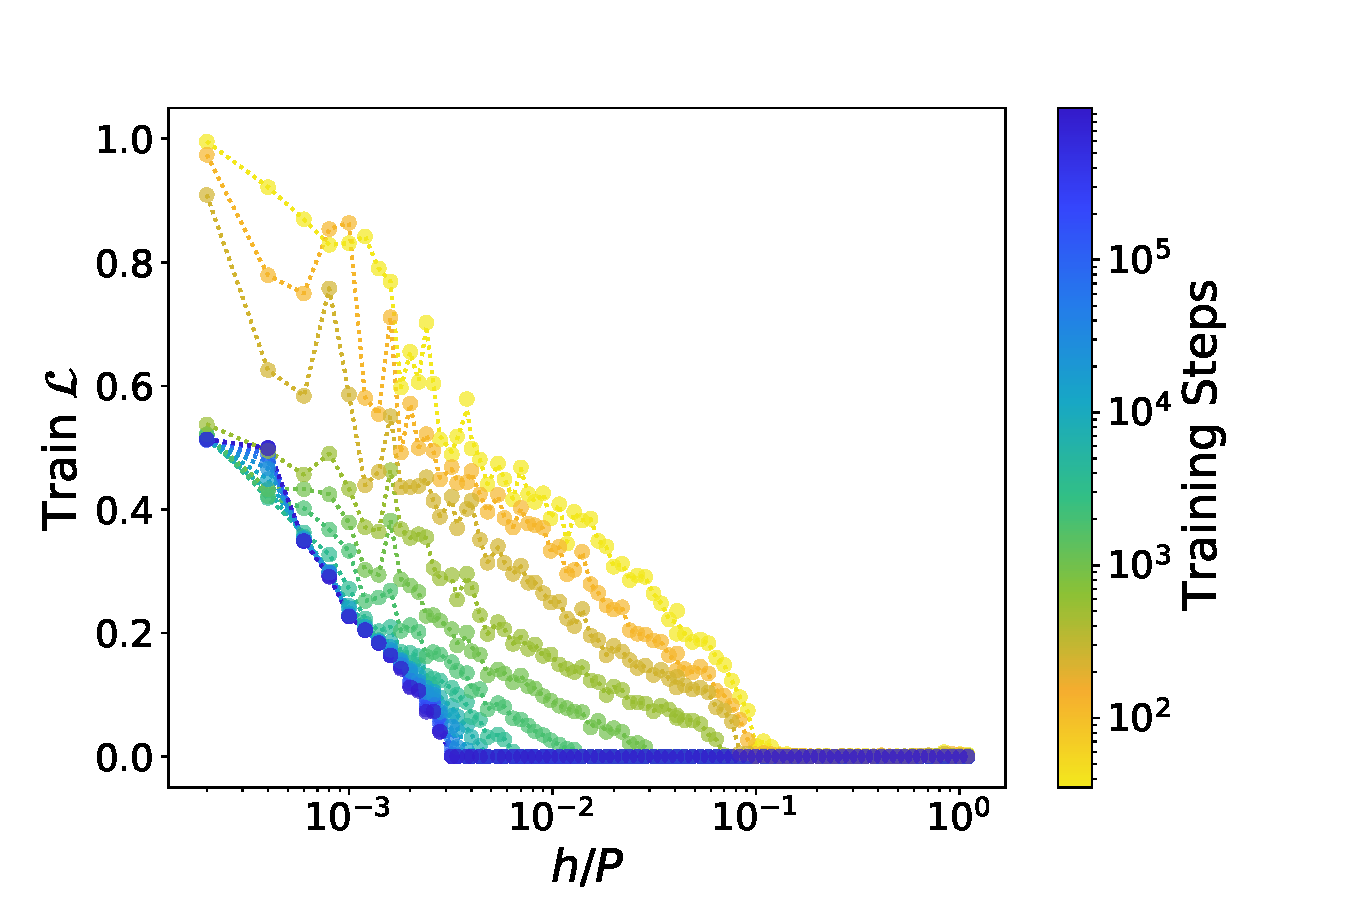
\includegraphics[width=\linewidth]{docs/assets/h_P_vs_train_loss_L=1_linear.pdf}
      \caption{}
    \end{subfigure}%
    \begin{subfigure}{.7\linewidth}
      \centering
      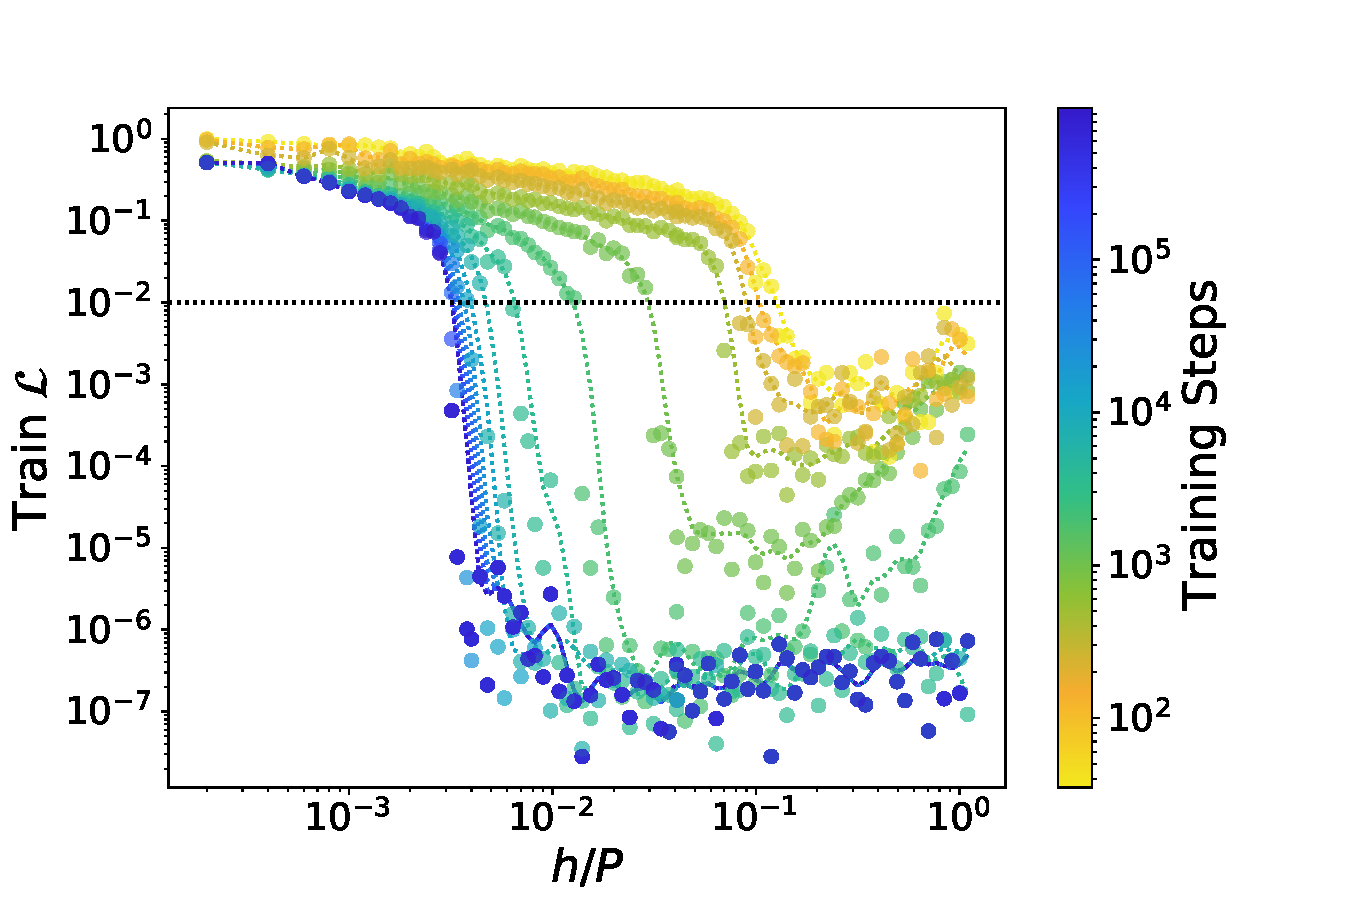
\includegraphics[width=\linewidth]{docs/assets/h_P_vs_train_loss_L=1_log.pdf}
      \caption{}
    \end{subfigure}
}\\
\caption{(a) Train loss $\mathcal{L}$ of the auxiliary model $\tilde f_t$ as a function of the over-parameterization ratio $h/P$, where $t$, measured in ``training steps," is distinguished by color. Points are connected with dotted lines to make it clear which data share the same value of $t$. Notice that as features move from lazy to learned, the number of features necessary to interpolate decreases. (b) Train loss is plotted on a logarithmic scale as a function of $h/P$. The horizontal dotted line corresponds to $\mathcal L_\text{train} = 10^{-2}$, an arbitrarily chosen threshold for use in determining $h^*$ which separates ``large" and ``small" loss values. For visual clarity in the noisy region with low loss, the dotted lines are smoothed with a Gaussian kernel.}
\label{h/P_vs_train_loss}
\end{figure}

We set an arbitrary threshold at $\mathcal L_\text{train} = 10^{-2}$ to separate the points that achieve a ``large" loss, corresponding to the under-parameterized regime, from those with ``small" loss, corresponding to the over-parameterized regime. This threshold is shown as a horizontal dotted line in Figure \ref{h/P_vs_train_loss}(b). As the present study only considers fixed value of $P$, we determine the location of the interpolation threshold in terms of $h$, but we expect the threshold to increase linearly in $P$ as was found by \cite{geigerJammingTransitionParadigm2019} and \cite{spiglerJammingTransitionOverparametrization2019}. This suggests that a future study that varies the value of $P$ should instead determine this threshold in terms of the density $h/P$. We identify the maximum value of $h$ for which the training loss is greater than or equal to the threshold value, denoting this critical value of $h$ as $h^*$. The value of $h^*$ as a function of the number of training steps taken by the feature model is shown in Figure \ref{h^*_vs_t}. $h^*$ decreases with the number of training steps before saturating to a minimum, corresponding to the convergence of the feature network as it optimizes. We remark on two compatible perspectives that can explain this decreasing behavior. The first is that we expect the trained features to contain more information about the response variable than the initial random features, thus requiring fewer auxiliary parameters to interpolate. The second perspective is that while the auxiliary model does not have direct access to the full parameter space of the feature model, more highly-trained features may correspond to an ``effective" number of parameters that is of order $N$, corresponding to the full parameter space of the feature model.\\

\begin{figure}[!h]
\centering
\captionsetup{width=.8\linewidth}
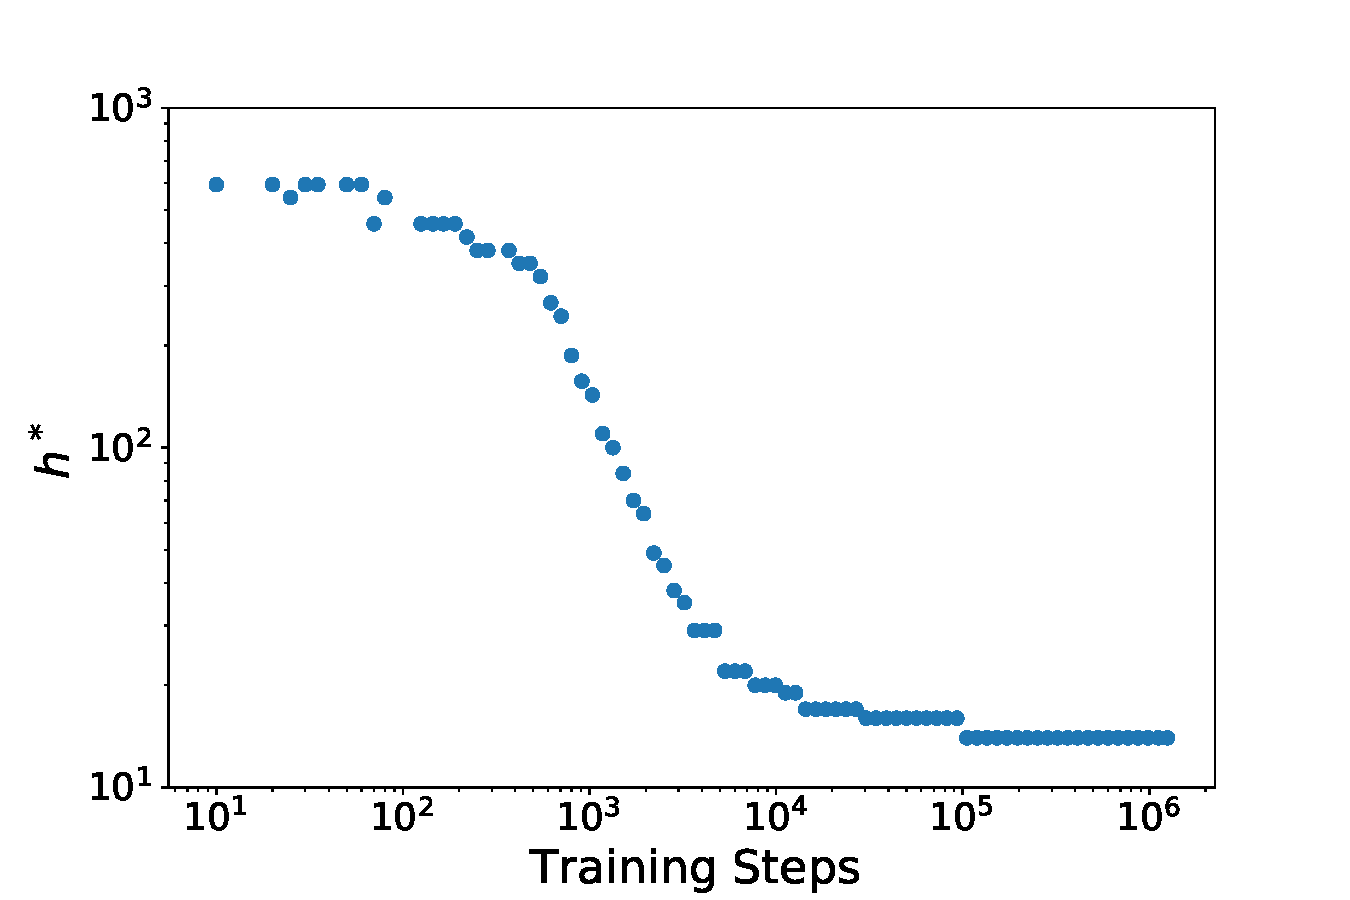
\includegraphics[width=.8\linewidth]{docs/assets/h_star_vs_train_steps_L=1.pdf}
\caption{$h^*$ as a function of the training steps of the feature network. The behavior is nearly monotonic and decreasing, saturating at a minimum value as the feature network converges.}
\label{h^*_vs_t}
\end{figure}

We further examine the behavior of the train loss by plotting it as a function of the re-scaled over-parameterization ratio $h/h^*$, shown in Figure \ref{h/h_star_vs_train_loss_log}. We can see that the loss follows a similar trajectory for all values of $t$ in the under-parameterized region before reaching a nearly vertical drop-off at the interpolation threshold, identified with $h/h^*=1$. The behavior at and beyond this threshold depends the degree of feature-learning, where the most highly-trained features are associated with the steepest and deepest drop-off. We hypothesize that this threshold will become increasingly steep and discontinuous as the number of training steps of the feature network go to infinity. \\

\begin{figure}[!h]
\centering
\captionsetup{width=.8\linewidth}
\centering
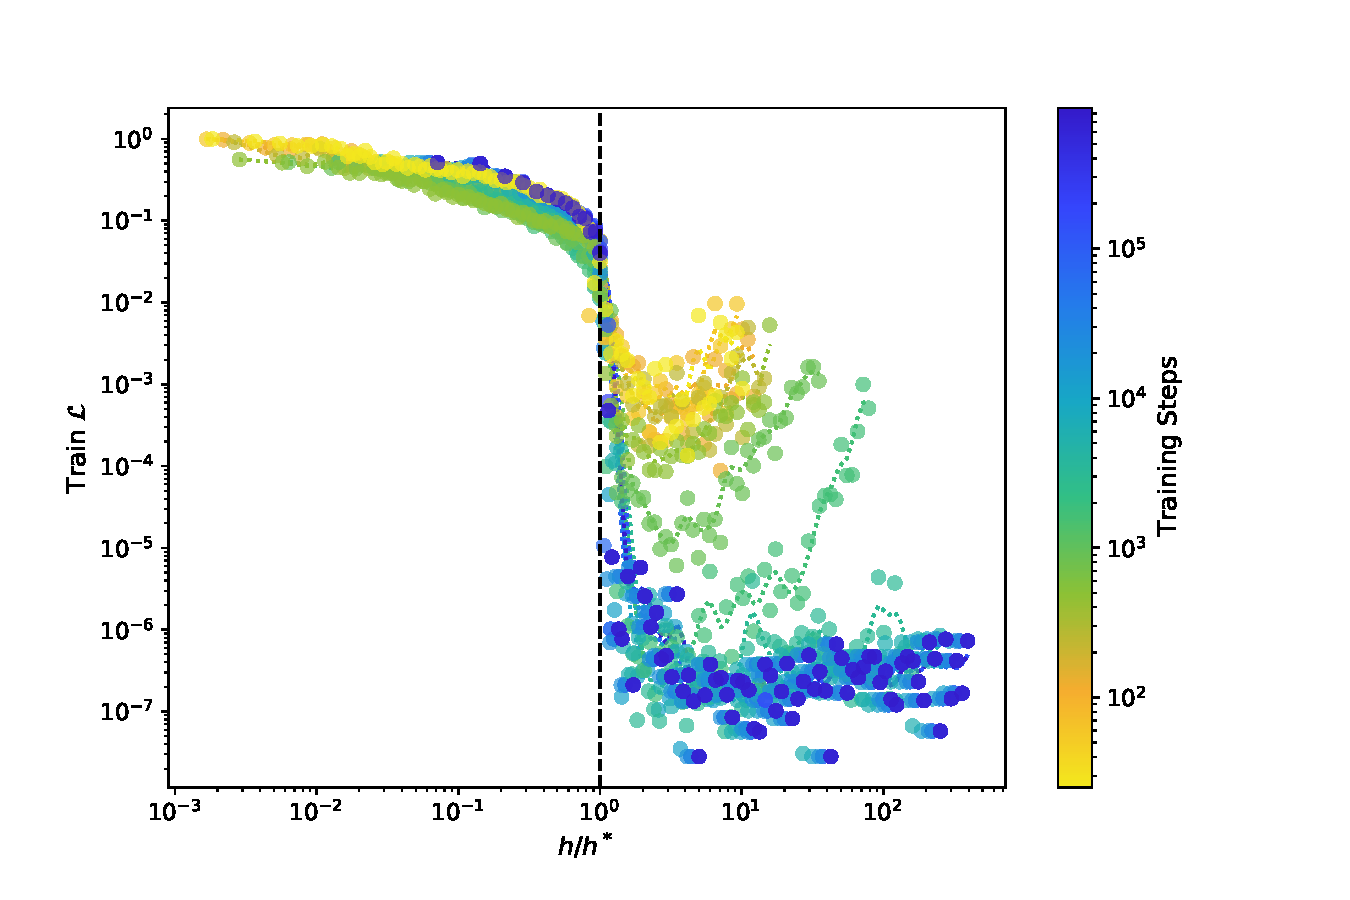
\includegraphics[width=.8\linewidth]{docs/assets/h_h_star_vs_train_loss_L=1_log.pdf}
\caption{Train loss plotted against re-scaled over-parameterization ratio $h/h^*$. The vertical dashed line at $h/h^*=1$ marks the interpolation threshold. Note that the transition is somewhat less sharp and less pronounced for lazy features than for trained features.}
\label{h/h_star_vs_train_loss_log}
\end{figure}

\subsection{Location of the Generalization Cusp}
A generalization cusp located at the interpolation threshold has been both predicted in analytic treatments of random features models \cite{meiGeneralizationErrorRandom2019}, \cite{dengModelDoubleDescent2020} and observed in empirical studies of real neural networks \cite{geigerJammingTransitionParadigm2019,spiglerJammingTransitionOverparametrization2019}. We therefore expect to observe peaks in the test loss $\mathcal L_\text{test} \equiv \mathcal L (\tilde f_t(\cdot, \hat 
a), \mathcal D_\text{test})$ in both models of random and trained features. Plotting the test loss as a function of $h/P$ does in fact display peaks with locations that decrease with the number of training steps, shown in Figure \ref{h/P_and_h_star_vs_test_loss_log}(a). In Figure \ref{h/P_and_h_star_vs_test_loss_log}(b), we can see that that these peaks occur at $h/h^*=1$, confirming the correspondence between the interpolation threshold and generalization cusp for lazy and trained features alike.

\begin{figure}[!h]
\centering
\captionsetup{width=.8\linewidth}
\makebox[\linewidth][c]{%
    \begin{subfigure}{.7\linewidth}
      \centering
      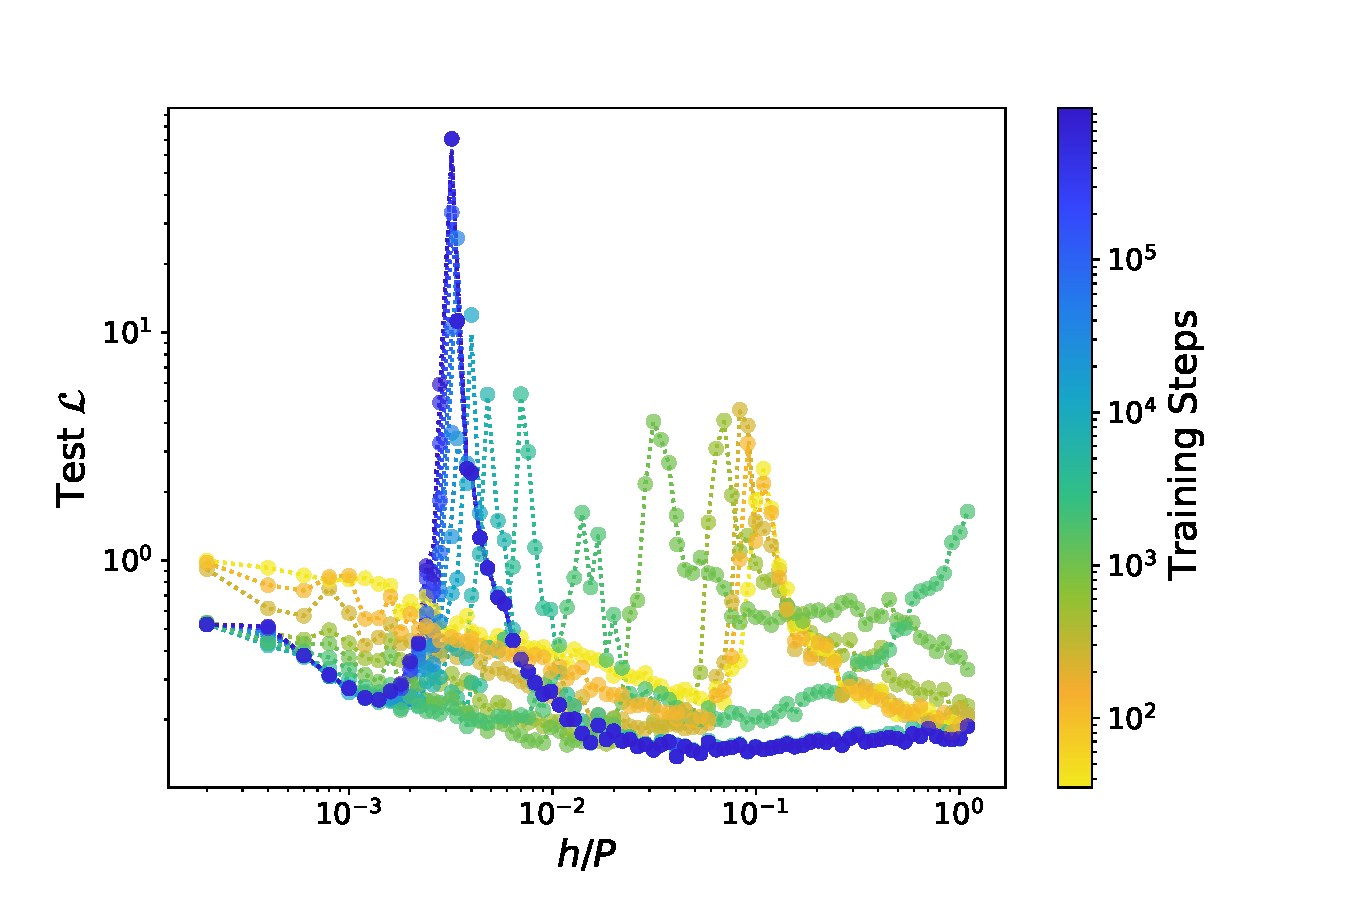
\includegraphics[width=\linewidth]{docs/assets/h_P_vs_test_loss_L=1_log.pdf}
      \caption{}
    \end{subfigure}%
    \begin{subfigure}{.7\linewidth}
      \centering
      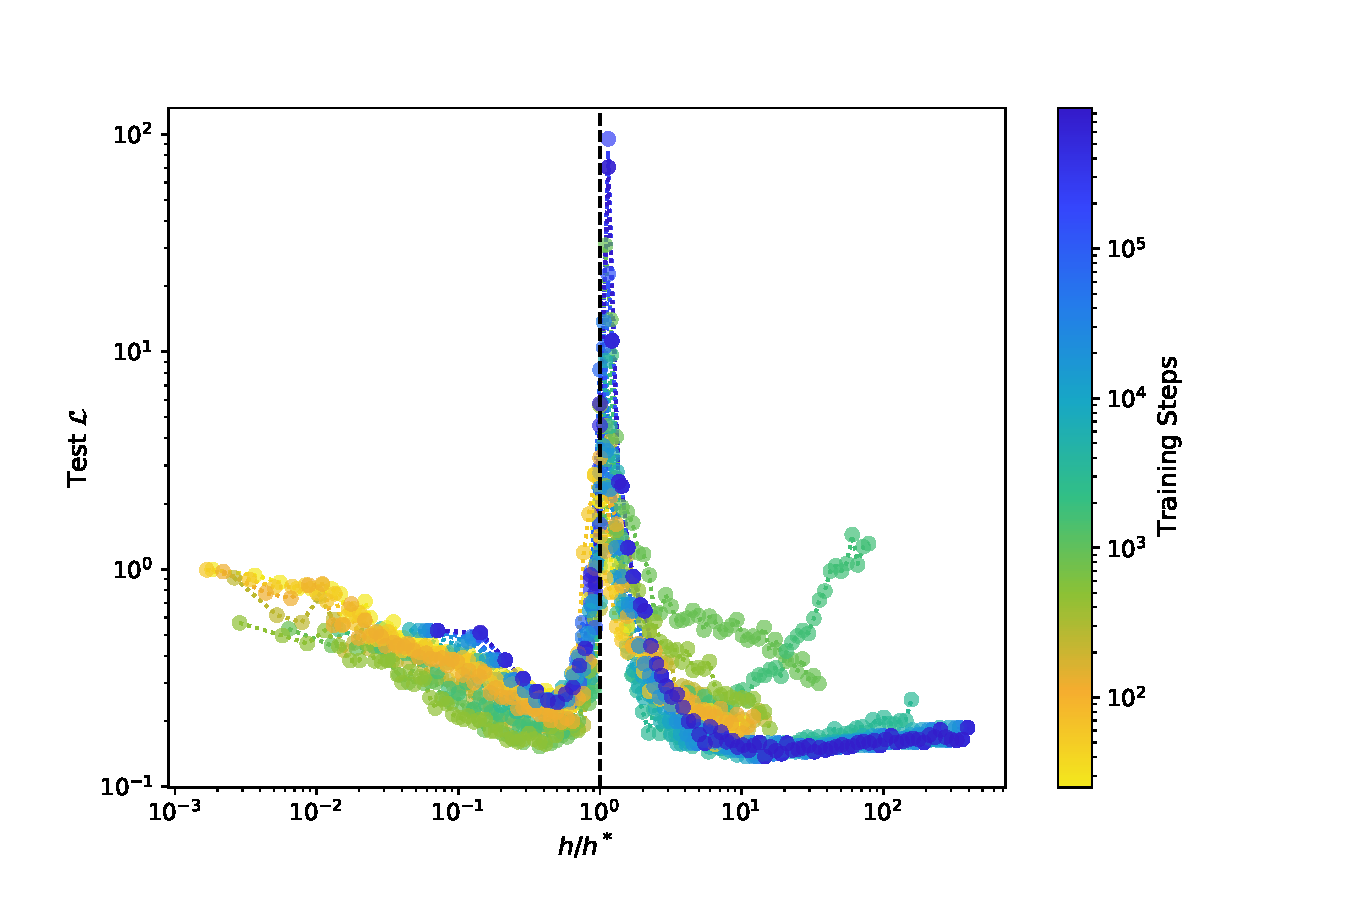
\includegraphics[width=\linewidth]{docs/assets/h_h_star_vs_test_loss_L=1_log.pdf}
      \caption{}
    \end{subfigure}
}\\
\caption{(a) Test loss is plotted as a function of $h/P$, showing sharp generalization cusps at values of $h/P$ that decrease in the number of training steps. (b) Test loss is plotted as a function of the re-scaled over-parameterization ratio $h/h^*$. The generalization cusps all align at $h/h*=1$, the location of the interpolation threshold.}
\label{h/P_and_h_star_vs_test_loss_log}
\end{figure}

\subsection{Location of Optimal Generalization}

In this section, we make some brief comments on the locations of the global minimizers of the test loss for different numbers of training steps observed in Figure \ref{h/P_and_h_star_vs_test_loss_log}(b). For both random and highly-trained features, this point occurs in the over-parameterized region $h/h^* > 1$, with the highly-trained features outperforming the random features at this point. Our study did not examine large enough values of $h$ to determine the behavior of the random features in the extremely far over-parameterized region, but the theoretical work of \cite{meiGeneralizationErrorRandom2019} and \cite{dengModelDoubleDescent2020} predict that generalization error should monotonically approach a minimum, potentially overtaking the models with highly trained features as was empirically found for FCNs in \cite{geigerDisentanglingFeatureLazy2020}. The models with moderately- to highly-trained features have test loss following a U-shaped curve in the over-parameterized regime, which is particularly harmful for the intermediately-trained features. It appears that the most highly-trained features are again becoming monotonic in this region, but precise determination of this behavior is outside the scope of this study and may form an interesting basis for further research. It is worth noting that a similar behavior is predicted by \cite{dengModelDoubleDescent2020} in the context of classification with random features and a simple feature-selection model, where the behavior in the overparameterized regime may be either monotonic or U-shaped depending on the choice of feature selection model.\\

\subsection{Jamming Phenomenology}
In this section, we present a numerical analysis of the qualitative behaviours of random and trained features in the vicinity of the interpolation threshold. The work of \cite{geigerJammingTransitionParadigm2019} and \cite{spiglerJammingTransitionOverparametrization2019} established a correspondence between the interpolation threshold in neural networks and a phase transition similar to the jamming phase transition observed in disordered solids, a hallmark of which is a discontinuous jump in the ratio of unsatisfied constraints to degrees of freedom. As the threshold is approached from above, this ratio jumps from a value of order zero to a value of order one. In order to examine the behavior of this ratio in our random and trained models, we need to more closely consider how the number of parameters should be counted. Although the auxiliary model has $h$ parameters, we expect trained features to contain more information about the response variables than random features, potentially taking advantage of all $N$ degrees of freedom of the feature model, and this expectation is supported by our finding that the interpolation threshold decreases with training. Therefore, we examine both the ratio $N_\Delta/h$ and $N_\Delta/N$ as functions of the re-scaled over-parameterization ratio $h/h^*$, expecting the former ratio to be the more relevant quantity for random features and the latter ratio to be more relevant for trained features. Because $N$ scales linearly in $h$ for $L=1$ and quadratically in $h$ for $L=2$, we examine $N_\Delta/h$ and $N_\Delta/N$ in both settings, as this difference in scaling has the potential to drastically affect our findings.\\

\begin{figure}[!h]
\centering
\captionsetup{width=.8\linewidth}
\makebox[\linewidth][c]{%
    \begin{subfigure}{.7\linewidth}
      \centering
      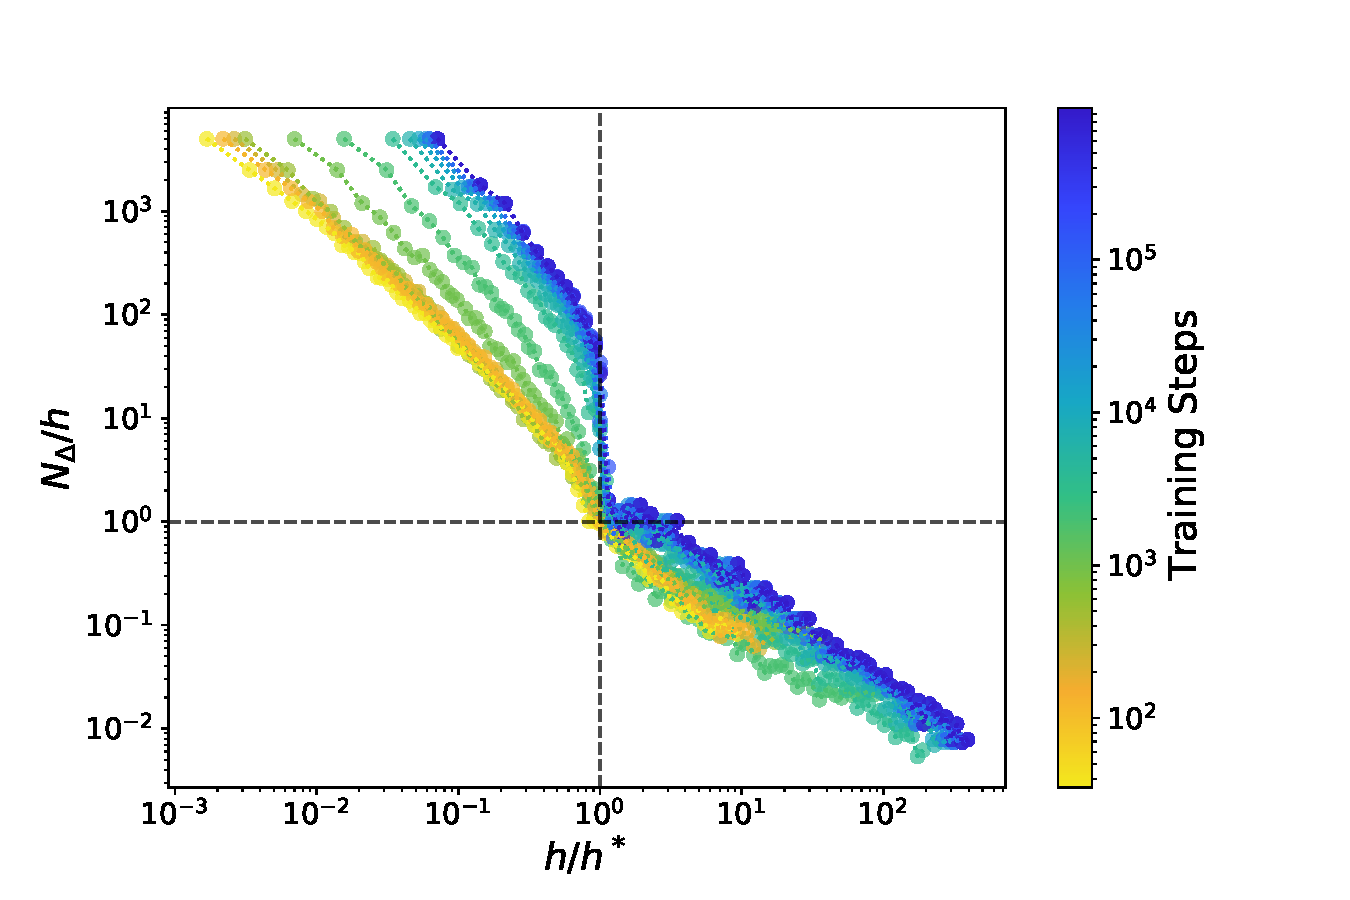
\includegraphics[width=\linewidth]{docs/assets/h_h_star_vs_N_del_h_L=1.pdf}
      \caption{$L=1, \ N_\Delta/h$}
    \end{subfigure}%
    \begin{subfigure}{.7\linewidth}
      \centering
      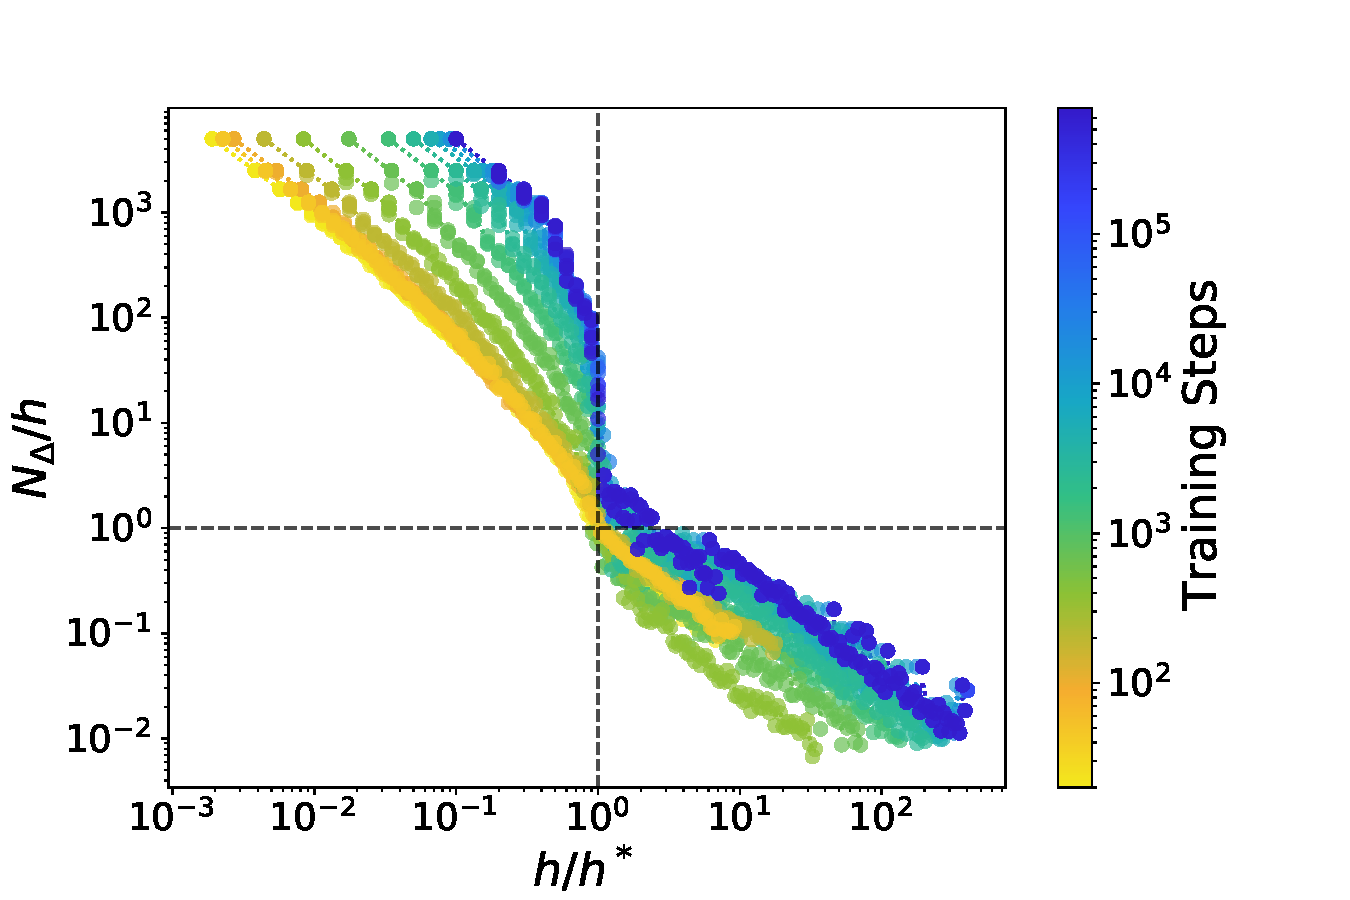
\includegraphics[width=\linewidth]{docs/assets/h_h_star_vs_N_del_h_L=2.pdf}
      \caption{$L=2, \ N_\Delta/h$}
    \end{subfigure}
}\\
\makebox[\linewidth][c]{%
    \begin{subfigure}{.7\linewidth}
      \centering
      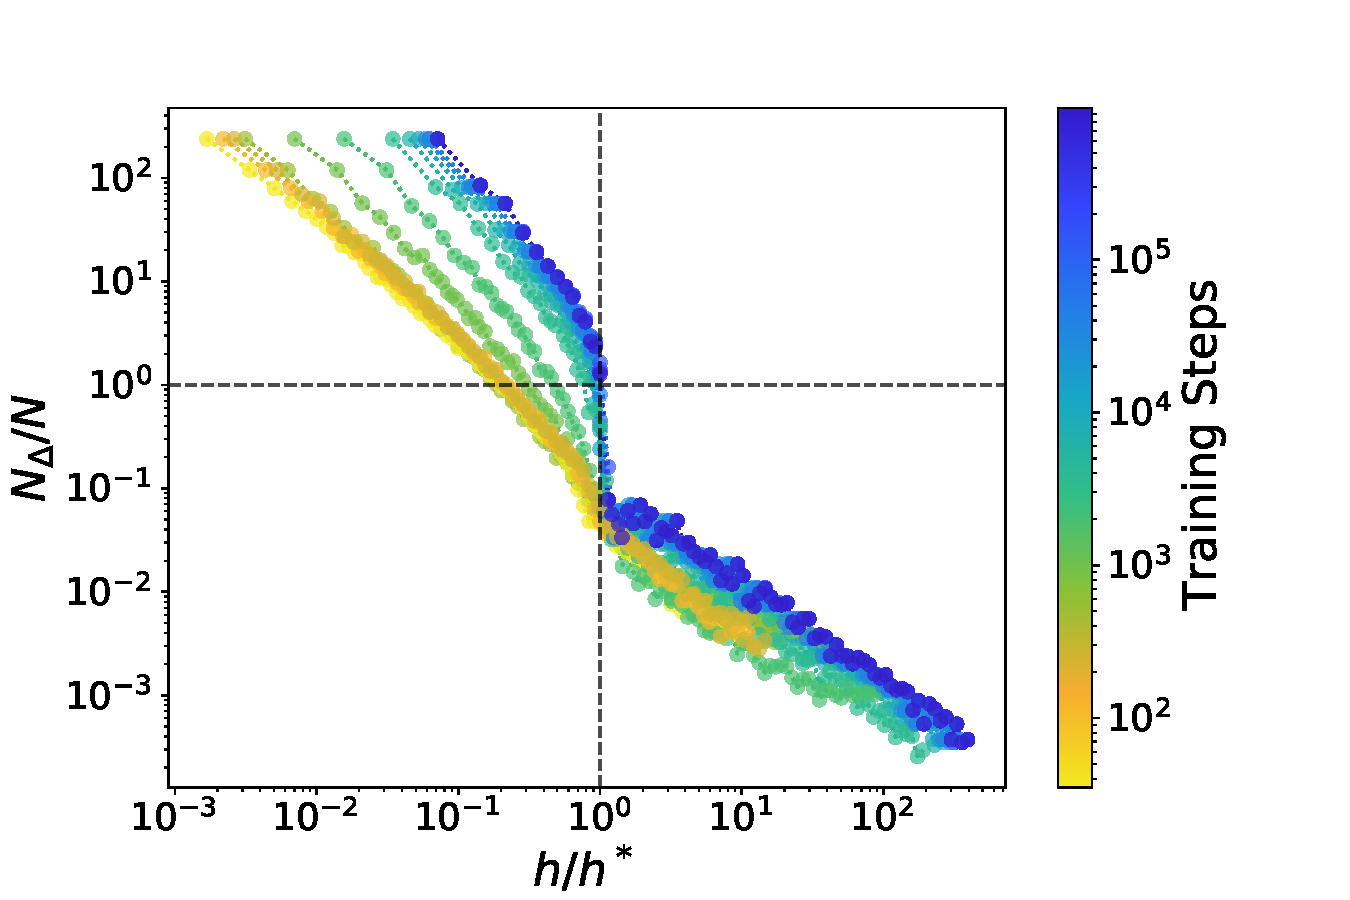
\includegraphics[width=\linewidth]{docs/assets/h_h_star_vs_N_del_N_L=1.pdf}
      \caption{$L=1, \ N_\Delta/N$}
    \end{subfigure}%
    \begin{subfigure}{.7\linewidth}
      \centering
      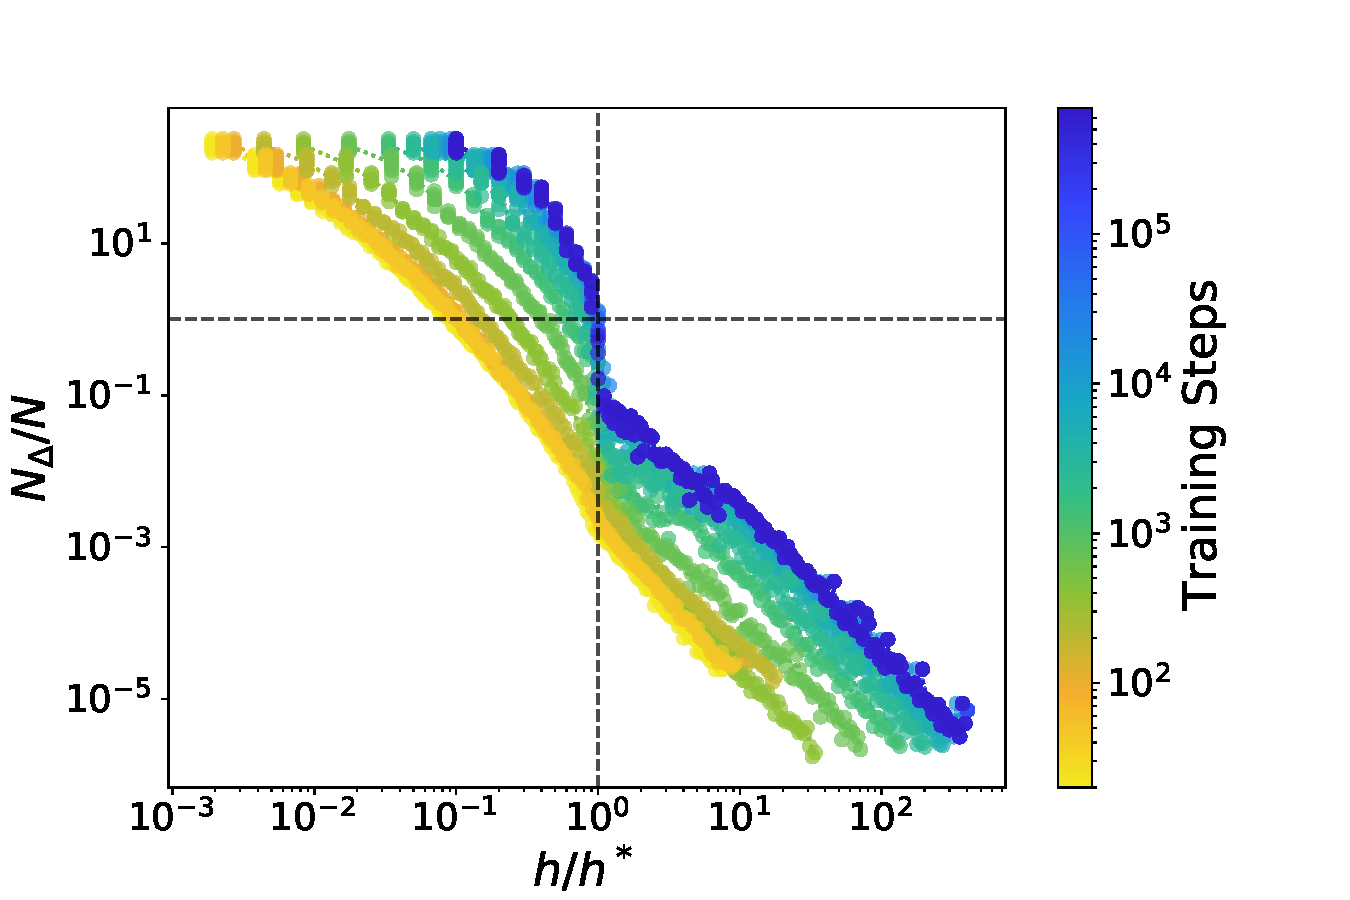
\includegraphics[width=\linewidth]{docs/assets/h_h_star_vs_N_del_N_L=2.pdf}
      \caption{$L=2, \ N_\Delta/N$}
    \end{subfigure}
}\\
\caption{Plotting $N_\Delta/h$ and $N_\Delta/N$ for $L=1$ and $L=2$ as functions of the re-scaled over-parameterization ratio $h/h^*$. Models with random features exhibit smooth behavior near the threshold at $h/h^*=1$ (vertical dotted lines), passing through $N_\Delta/h=1$. Models with highly trained features exhibit nearly discontinuous behavior, jumping from approximately $N_\Delta/h=1$ (horizontal dotted line in (a, b)) to $N_\Delta/N=1$ (horizontal dotted line in (c, d)).}
\label{N_del_discontinuity}
\end{figure}

Examining the way $N_\Delta/h$ depends on $h/h^*$ in models with randomly initialized features, we find no evidence of jamming. Figure \ref{N_del_discontinuity}(a) and \ref{N_del_discontinuity}(b) show $N_\Delta/h$ as a function of $h/h^*$ for $L=1$ and $L=2$, respectively. The points corresponding to the models with randomly initialized features (yellow) trace out a curve that passes directly through the intersection of $h/h^*=1$ and $N_\Delta/h=1$. This curve is smooth over its whole domain, save for a slight inflection at the threshold, and exhibits no discontinuities that would be indicative of jamming. Models with highly-trained features, however, tell a different story. Figure \ref{N_del_discontinuity}(a) and \ref{N_del_discontinuity}(b) show the points corresponding to these models (blue) passing near the intersection of $h/h^*=1$ and $N_\Delta/h=1$, just as we observed for random features, but we note that this behavior is less precise for $L=2$, where they cross $N_\Delta/h=1$ at a value of $h/h^*$ that is slightly greater than one. A far more striking behavior, however, is that as $h/h^*=1$ is approached from the over-parameterized region, the curve exhibits a near-discontinuity, jumping from $N_\Delta/h\approx1$ to a value that is one to two orders of magnitude larger. Figure \ref{N_del_discontinuity}(c) and \ref{N_del_discontinuity}(d), which instead plot $N_\Delta/N$ as a function of $h/h^*$, show that the upper end of the jump is located at approximately $N_\Delta/N = 1$ for both $L=1$ and $L=2$. Because $N$ scales as $O(d\cdot h)$ for $L=1$ and $O(h^2)$ for $L=2$, the consistency of this behavior across the two scaling conditions is strong evidence that the jump from $N_\Delta/h \approx 1$ to $N_\Delta/N \approx 1$ is systematic rather than coincidental. If we assume that the effective number of parameters ``$N_\text{eff}$" in the models with highly-trained features is approximately equal to $N$, then this corresponds to a jump from $N_\Delta / N_\text{eff} \approx 1/d$ to $N_\Delta / N_\text{eff} \approx 1$ for $L=1$ and a jump from $N_\Delta / N_\text{eff} \approx 1/h$ to $N_\Delta / N_\text{eff} \approx 1$ for $L=2$. Recall that for a model with $N$ degrees of freedom, the jamming transition is characterized by a jump from $N_\Delta/N = O(0)$ to $N_\Delta/N = O(1)$ at the interpolation threshold. The jump we observe for the trained-feature models is consistent with this characterization of jamming, so long as $d$ and $h$ are taken to be large. The $O(1/d)$ and $O(1/h)$ scaling that we observe offers a potential refinement of the findings of \cite{geigerJammingTransitionParadigm2019} and \cite{spiglerJammingTransitionOverparametrization2019} for the magnitude of $N_\Delta/N$ as the threshold is approached from the right. \\

Surprisingly, the jamming we observe in this context bears similarities to an isostatic jamming transition rather than to the hypostatic jamming transition previously observed in neural networks. While the hypostatic transition is characterized by a jump to $N_\Delta/N = c$ where $c < 1$ is a finite, order one quantity, the isostatic transition is characterized by a jump to $N_\Delta/N=1$, as we have observed here. Jamming is isostatic in the convex perceptron and hypostatic in the non-convex perceptron \cite{franzSimplestModelJamming2016}, suggesting that the hypostatic behavior we observe is due to the convexity of the auxiliary loss for fixed features. However, the auxiliary model is only convex in the $h$ auxiliary parameters and not in the $N-h$ parameters before the last hidden layer of the feature network, so this explanation is not entirely satisfactory in explaining the hypostatic jamming over all $N$ parameters.\\

% \subsection{The Effects of Regularization in Lazy and Learned Features}
% \label{regularization}
% TODO IF TIME. Worst case, I can drop this section without too much worry.\\

\section{Discussion}
\label{Discussion}

The main purpose of this study is to examine some of the similarities and differences between the lazy- and feature-learning regimes. While lazy learning has proven to be an effective framework for explaining a number of the convergence and generalization properties of neural networks, it describes a regime of learning that is distinct from feature learning. We cannot naively extend insights from one regime to another. Feature learning is still poorly understood, but it has been implicated as a key component to the successes of some of the most effective neural architectures. It is important that we develop models for characterizing the convergence and generalization abilities of networks in this regime so that we can engineer new architectures that take full advantage of these properties. Understanding the similarities and differences between these two regimes will be key in extending the models that have successfully been used to describe lazy learning, such as the ``random-feature" model, to the feature-learning setting. By beginning with random features and ``training" them with a feature network, we attempt to probe some of the differences that emerge as training converges. We in particular examine these differences in the vicinity of the interpolation threshold, a point associated with critical behavior of both network convergence and generalization.\\

\subsection{Summary of Main Results} 

For both lazy and learned features, we observe a cusp in the generalization error at the interpolation threshold, which is consistent with previous empirical studies and theoretical predictions. Despite this critical behavior at the threshold, we found no evidence of jamming in the lazy-learning regime. For random features, the ratio of unsatisfied constraints to auxiliary parameters $N_\Delta/h$ varies smoothly across the interpolation threshold, showing none of the tell-tale signs of jamming. On the other hand, jamming phenomenology is recovered as features are progressively trained: $N_\Delta/h$ becomes steeper at the threshold, exhibiting a near-discontinuity by the end of training.\\

Previous literature has not explicitly distinguished between the jamming transition and the generalization cusp in neural networks; however, our findings show that although both phenomena occur at the interpolation threshold, they are distinct phenomena, and the generalization cusp can occur without jamming. Understanding the mechanisms which cause jamming to emerge in the feature-learning regime but not in the lazy regime may lead to deeper insights about how feature learning behaves both near and beyond the threshold and how to model generalization in this setting.\\

\subsection{Limitations and Critical Analysis}

The core assumption of this study is that linear models over the activations of a neural network capture the crucial aspects of feature learning as the neural network undergoes training. There is a clear correspondence between linear models over the final-layer activations of a randomly-initialized feature network and a network training in the lazy regime. However, it is unclear whether training the feature network is a suitable model of feature learning in typical neural networks.\\

In this study, we considered linear models over the $h$ features generated by the final layer of an $N$-parameter feature network. At initialization, this model is equivalent to an $h$-parameter lazy neural network. When the feature-model is nearing convergence, however, we observed evidence that the effective number of parameters approaches $N$. Although one might expect a model with feature learning to be more expressive than one without, it is unclear whether the observed increase in the effective degrees of freedom is a contrived consequence of our specific modeling choices, or if it is a reflection of a more general phenomenon. It may be worth exploring whether networks that undergo feature-learning have an effective number of parameters that is higher than a lazy network of the same size and architecture. Because it is possible to force feature learning or lazy learning with an appropriate scaling choice on the weights of the final layer \cite{chizatLazyTrainingDifferentiable2020,geigerDisentanglingFeatureLazy2020}, a future study could clarify some of these questions and uncertainties by training networks in each regime directly, avoiding the need for an auxiliary model and a feature model.\\ 

A further limitation to our study is that we only examined a single data-set, MNIST, with a fixed number of training data, $P=5000$. The generalization capabilities of random-features models in the vicinity of the interpolation threshold depends strongly on the structure of the data, and in particular the signal to noise ratio of the target variables \cite{meiGeneralizationErrorRandom2019}. Whether lazy or feature learning generalize better has also been shown to depend on data structure \cite{geigerDisentanglingFeatureLazy2020}. Although it is beyond the scope of this study, it is therefore important to consider the affect that data-set choice has on the behaviors of networks undergoing lazy or feature learning.

\subsection{Conclusion}

We have found that although both lazy learning and feature learning exhibit generalization cusps at the interpolation threshold, only feature learning exhibits a jamming transition at this point. Identifying such a difference may be an important step towards understanding feature learning, but there are a number of open questions that need to be answered before this finding can be taken advantage of. What is the role of feature learning in the emergence of jamming phenomenology? What does the presence of jamming in one regime but not the other tell us about how convergence and generalization differ across these settings? Answering these questions may fill some important gaps in our understanding of neural networks, allowing practitioners to design better architectures that most efficiently generalize from data. \\
 
\printbibliography
\newpage
\thispagestyle{empty} 
\section*{Self assessment}
\vspace{1cm}
\begin{center}
\begin{tabular}{ |c|c|L| } 
 \hline
 Category & Score & Comments \\ 
 \hline
 \hline
 Scientific quality & 68 & I feel that I could have gone a bit deeper with some of the mathematical aspects of this all. I am somewhat disappointed because I also did additional analyses, including looking into the effects of regularization, that did not make it into the final report. The writing process was a lot more difficult than I expected, and I did not have time to integrate this information here. This all being said, I still think that my experiments and critical analyses are of high quality\\ 
 \hline
 Breadth & 96 & Almost none of the information in this domain was covered in my coursework, and I was only able to put all of this information together with \textit{extensive} reading. \\ 
 \hline
 Originality & 92 & This work also took a lot of synthesis. Knowing what I know now, none of this feels very original. However, I only know what I know now due to my own creative exploration and work in connecting the dots of all of the reading that I did. \\ 
 \hline
 Presentation & 70 & I feel that I presented my work in a logical manner that conveys my findings well and is easy to read. I am happy how this has all turned out.\\ 
 \hline
\end{tabular}
\end{center}

\end{document}